\subsection{Prueba de rendimiento en teléfono \textit{Huawei TAG-L13}}
Esta prueba se realiza una vez que hechas las modificaciones como producto de las pruebas unitarias, de integración y de sistema.
\subsubsection{Objetivo de la prueba}
Verificar el uso del GPU y el nivel de batería del teléfono que utiliza mientras la aplicación esté funcionando.
\subsubsection{Herramientas utilizadas durante la prueba}
Opciones de desarrollador del teléfono Huawei TAG-L13 y \textit{Battery Doctor}.
\subsubsection{Aplicación de la prueba}
Para esta prueba se debe de instalar la apk del juego en el dispositivo, activar las
opciones de desarrollador e instalar la aplicación \textit{Battery Doctor}.  Una vez
hecho esto se juega el juego y se mide el desempeño desde el teléfono. En las figura
\ref{fig:GPUHuawei} se muestra el uso del GPU en distintos momentos de la
partida. Por otra parte en la figura \ref{fig:BateriaYolotl} se muestra el uso
de la batería y el uso promedio de \textit{GPU} que mide \textit{Battery Doctor}.
\\
\par
\begin{figure}
  \centering
 
   \subfigure[Uso del GPU desde el menú principal.] {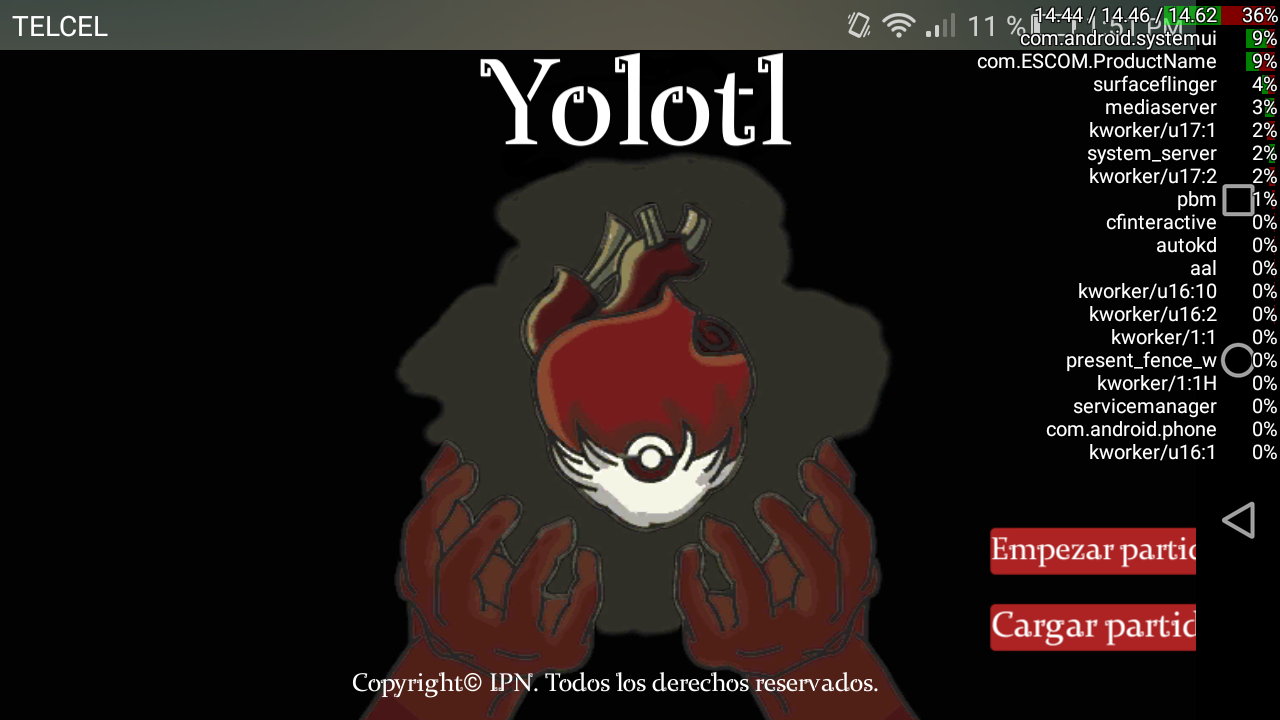
\includegraphics[width=0.4 \textwidth]{04ResultadosObetnidos/imagenes/rendimiento01.png}}
   
   \subfigure[Uso del GPU desde el menú de selección de nivel.] {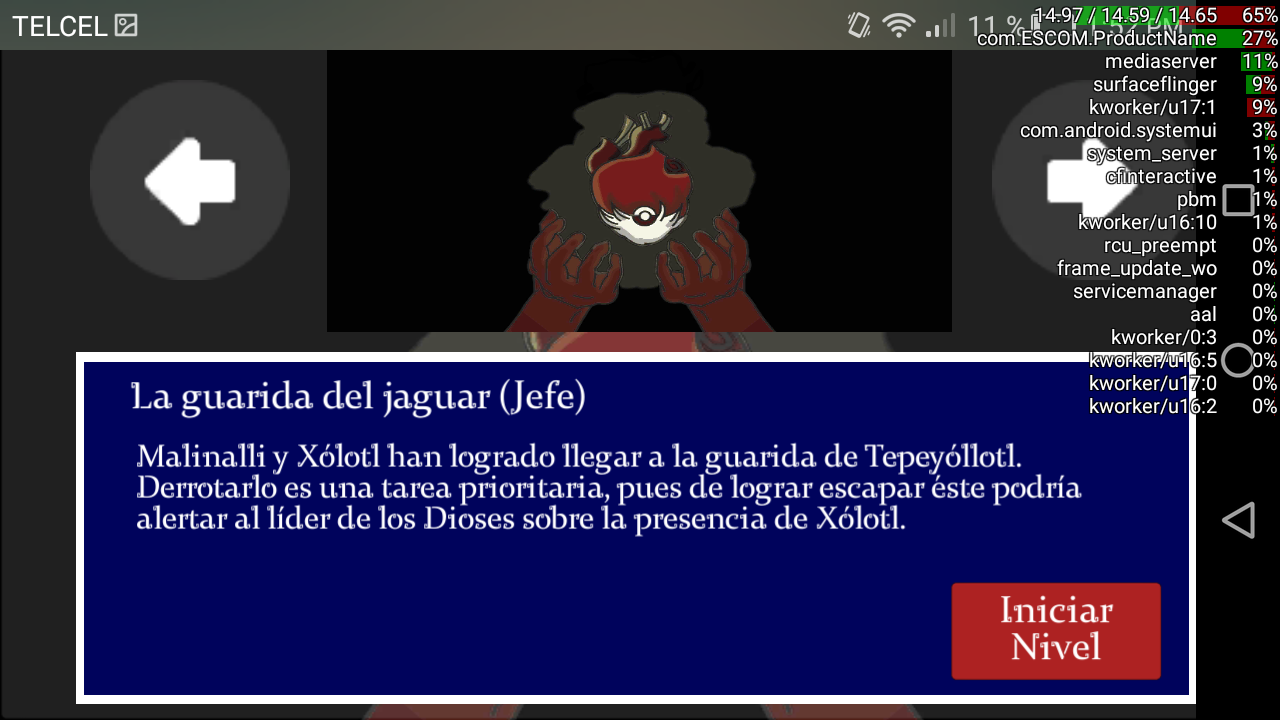
\includegraphics[width=0.4 \textwidth]{04ResultadosObetnidos/imagenes/rendimiento02.png}}
   
   \subfigure[Uso del GPU desde una cinemática.] {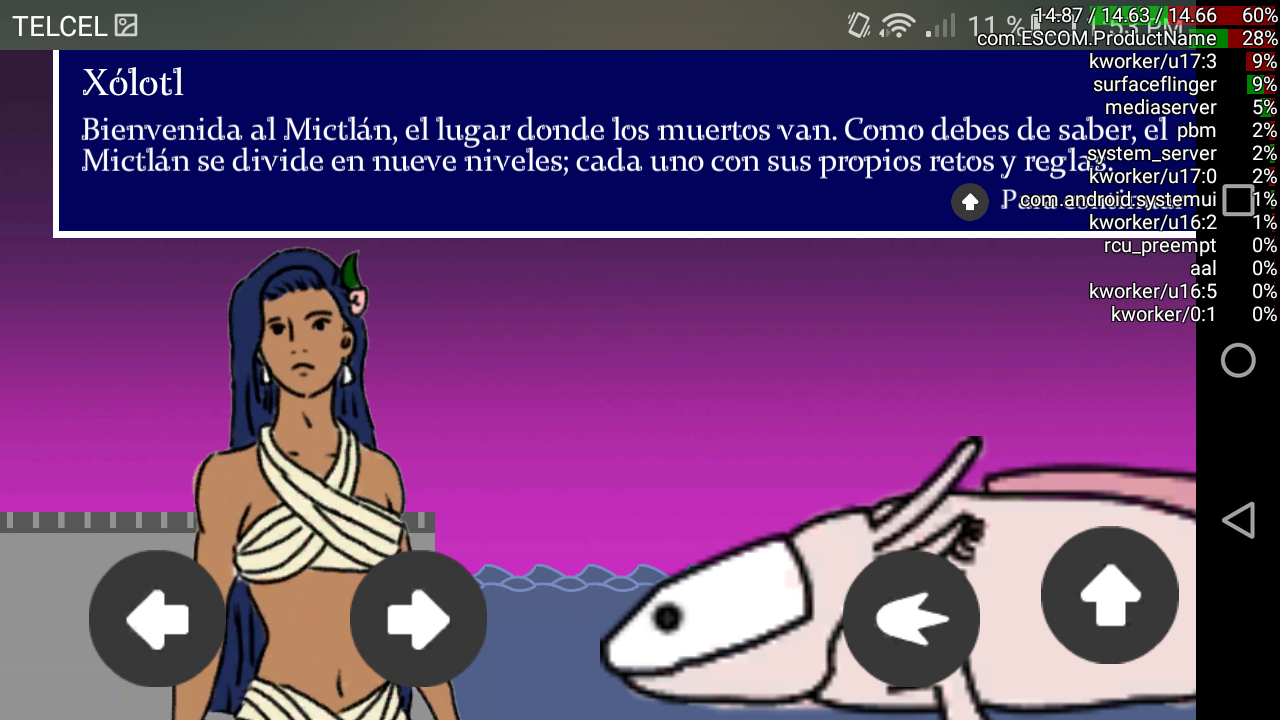
\includegraphics[width=0.4 \textwidth]{04ResultadosObetnidos/imagenes/rendimiento03.png}}
   
   \subfigure[Uso del GPU desde un nivel de plataforma.] {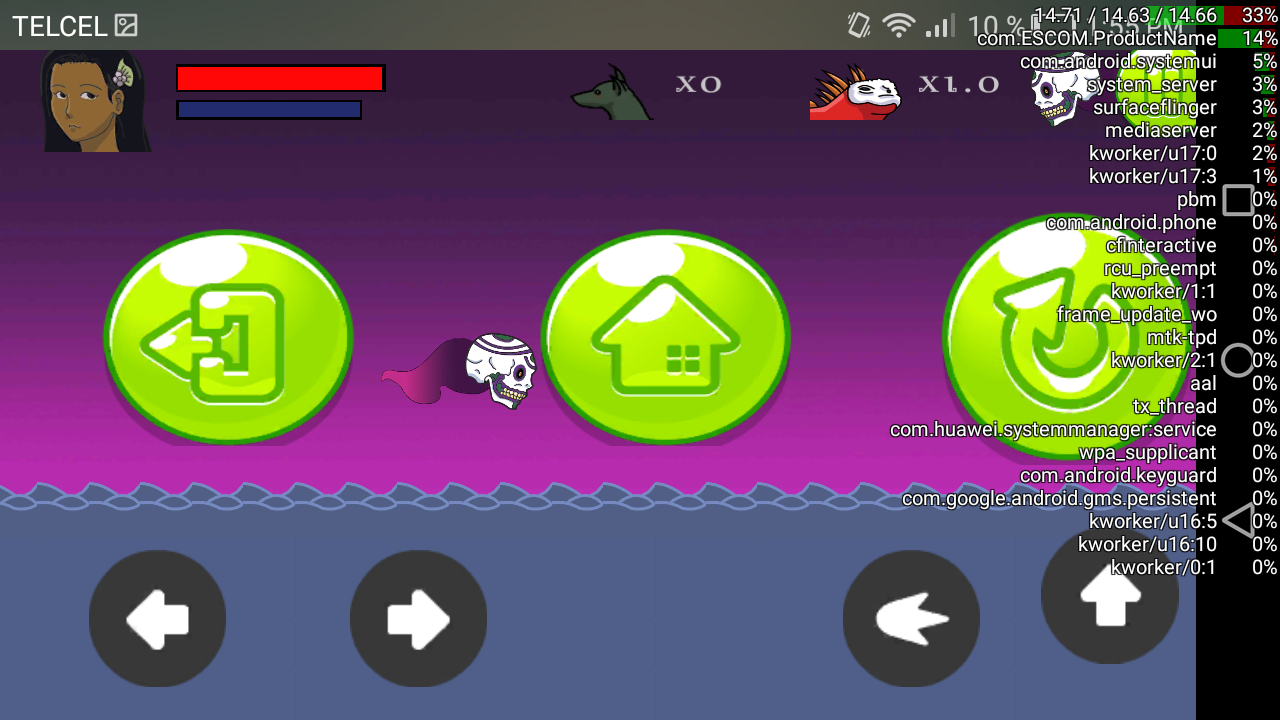
\includegraphics[width=0.4 \textwidth]{04ResultadosObetnidos/imagenes/rendimiento05.png}}
   
   \subfigure[Uso del GPU desde un nivel de jefe.] {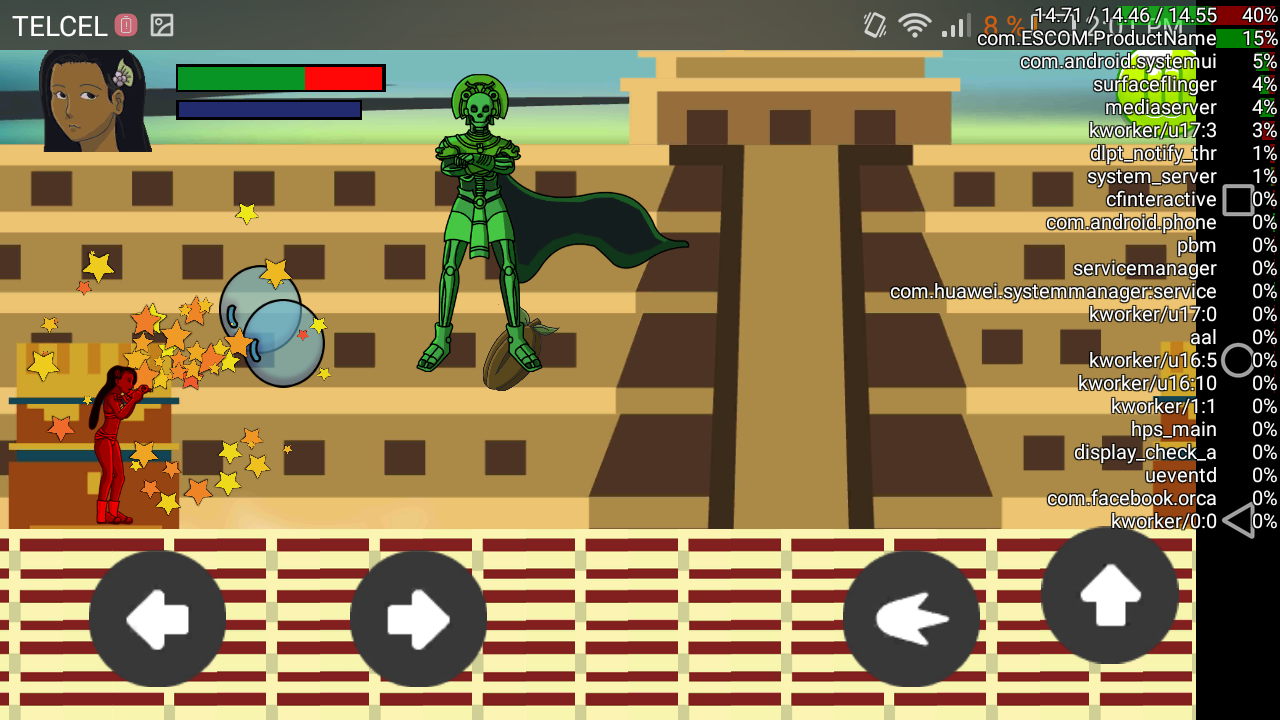
\includegraphics[width=0.4 \textwidth]{04ResultadosObetnidos/imagenes/rendimiento10.png}}
   
  \caption{Resultados del rendimiento del GPU del dispositivo Huawei}
  \label{fig:GPUHuawei}
\end{figure}
                \begin{figure}[h]
                        \centering
                        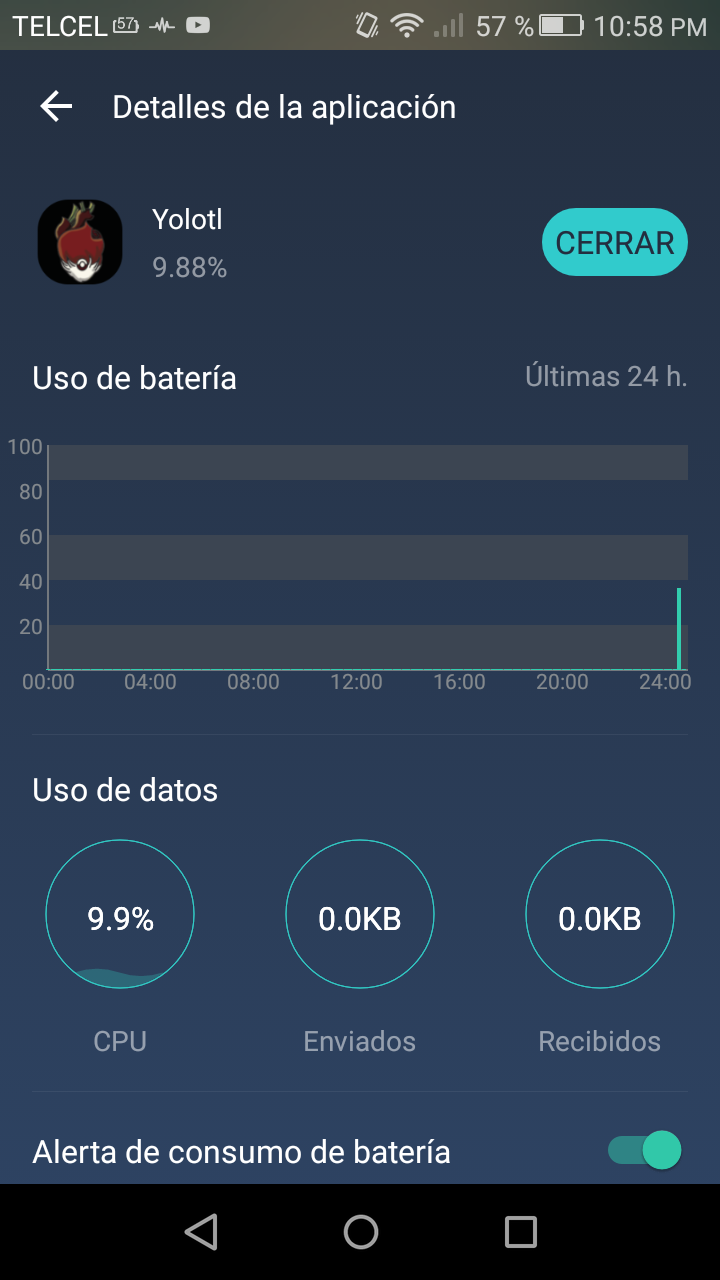
\includegraphics[width=0.2\textwidth]{04ResultadosObetnidos/imagenes/baterry02.png}
                        \caption{Pantalla de la aplicación \textit{Battery Doctor} para medir el
                        rendimiento del juego.}
                        \label{fig:BateriaYolotl}
                \end{figure}
\subsubsection{Conclusiones de la prueba}
De esta medición del desempeño del GPU se puede observar que la aplicación
utiliza un mínimo del 9\% del GPU y hasta un máximo del casi el 30\%. Por su
parte, el juego utiliza en promedio un 40\% de la batería. Estas cifras son
buenas si se considera que otras aplicaciones como \textit{Messenger} de
\textit{Facebook} llega a utilizar el 50.6\% del GPU y casi el 60\% de la batería
del teléfono, ver figura \ref{fig:BateriaFacebook}.
\begin{figure}[h]
                        \centering
                        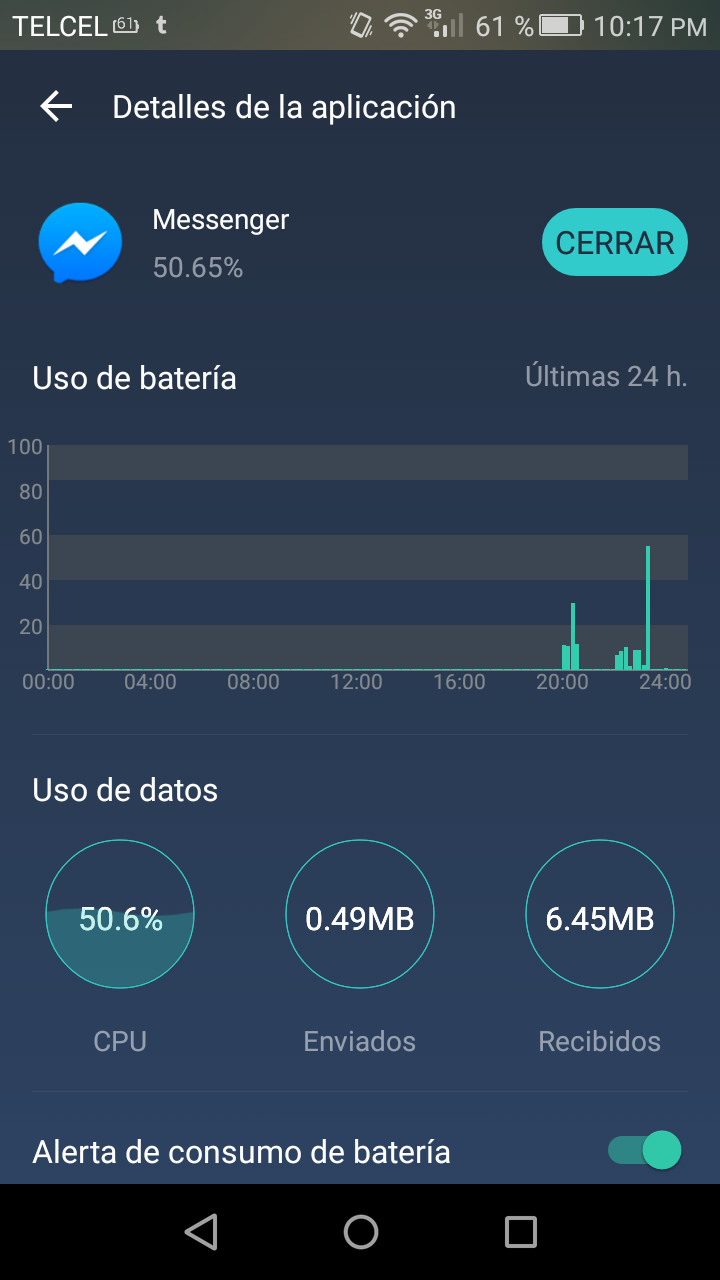
\includegraphics[width=0.2\textwidth]{04ResultadosObetnidos/imagenes/baterry01.png}
                        \caption{Pantalla de la aplicación \textit{Battery Doctor} para medir el
                        rendimiento de \textit{Messenger} de \textit{Facebook}.}
                        \label{fig:BateriaFacebook}
                \end{figure}